\documentclass[]{final_report}
\usepackage{graphicx}
\usepackage{hyperref}


%%%%%%%%%%%%%%%%%%%%%%
%%% Input project details
\def\studentname{Ciaran Palmer}
\def\projecttitle{SensorML on SenseTile}
\def\supervisorname{Your Supervisor Name}
\def\moderatorname{Your Moderator Name}


\begin{document}

\maketitle
\tableofcontents\pdfbookmark[0]{Table of Contents}{toc}\newpage

%%%%%%%%%%%%%%%%%%%%%%
%%% Your Abstract here

\begin{abstract}
SenseTileSensor Board

SensorML description.

WebServer to access sensor observations

SensorML Bon Mapping with a tool and method to develop sensorML descriptions

\end{abstract}




\newpage


%%%%%%%%%%%%%%%%%%%%%%
%%% Acknowledgments

\chapter*{Acknowledgments}


%%%%%%%%%%%%%%%%%%%%%%
%%% Introduction

\chapter{Introduction}

The aim of this thesis project was to prototype a Web Service for accessing sensor observations from the SenseTile Sensor Board. SenseTile is a sensor and processing package including motion sensors, RFID sensors, temperature sensor, audio sensors, pressure sensors, light level sensors video sensors among others. It is used as a replacement for standard ceiling tiles to provide smart building services as part of a Web Sensor Network.

Descriptions of the SenseTile Sensor Board were to be developed using Sensor Model Language (SensorML)\cite{SensoMLref}. SensorML is a language that describes the process of sensor measurement by providing standard models and XML encoding for such processes. SensorML was be used as it is becoming a standard for describing sensor data processing as part of the SWE.

Another part of the thesis was to define a SensorML to BON Mapping . BON\cite{BONref} is a notation and a method for Object Oriented systems analysis and design. Based on this mapping it was proposed to develop a tool/method to automatically generate SensorML descriptions. Generally SensorML is hand generated with all the shortcomings of such an approach. The proposed approach would allow sensor processing to defined formally in BON and then refined to JML/Java. 


\chapter{ Background Research}

How was problem solved before.


\chapter{SensorML}
\section{SensorML Overview}
The Open Geospatial Consortium (OGC) Sensor Web Enablement (SWE) activity, is being executed through the OGC Web Services (OWS) initiatives (under the Interoperability Program). The SWE initiatives are establishing the interfaces and protocols that will enable a “Sensor Web” through which applications and services will be able to access sensors of all types over the Web.
All processes define their inputs, outputs, parameters, and method, as well as provide relevant metadata. SensorML models detectors and sensors as processes that convert real phenomena to data.

sensors modeled as processes that can be connected and participate equally within a process chain or system, and which utilize the same process model frame as any other process.
Processes are entities that take one or more inputs and through the application of well-defined methods using specific parameters, results in one or more outputs.  SensorML also supports linking between processes and thus supports the concept of process chains, which are themselves defined as processes.
The second possible role is to provide processing chains with which SensorML-enabled software could derive new data from existing observations on-demand.

A standard description format for sensors is important for the long-term definition of the sensor model’s fundamental characteristics and assumptions for use in future reprocessing and refining of sensor data.

a System defines a collection of sensors that are related spatially and temporally to one another, as well as related to some geospatial domain.
Detectors are typically simple devices (real or virtual) that take one input signal and generate one or more output signals.

In SensorML, these simpler atomic processes are defined as “process models”, if they are pure processes with no real connection to a spatial or temporal domain, and as “components” if they are physical processing devices, such as detectors and actuators.

SensorML is mostly used to describe functional models of the sensors rather than the hardware.

The response characteristics of a sensor determine how the sensor will react to a particular stimulus (i.e., phenomenon) and how it will operate under given environmental conditions. Within the sensor response characteristics will be specifications for sensitivity (e.g., threshold, dynamic range, capacity, band width, etc.), accuracy and precision, and behavior under certain environmental conditions.

    Component -

    Physical atomic process that transforms information from one form to another. For example, a Detector typically transforms a physical observable property or phenomenon to a digital number. Example Components include detectors, actuators, and physical filters.

    System -

    Composite physically-based model of a group or array of components, which can include detectors, actuators, or sub-systems. A System relates a process to the real world and therefore provides additional definitions regarding relative positions of its components and communication interfaces.

    Process Model -

    Atomic non-physical processing block usually used within a more complex Process Chain. It is associated to a Process Method which defines the process interface as well as how to execute the model. It also precisely defines its own inputs, outputs and parameters.

    Process Chain -

    Composite non-physical processing block consisting of interconnected sub-processes, which can in turn be Process Models or Process Chains. A process chain also includes possible data sources as well as connections that explicitly link input and output signals of sub-processes together. It also precisely defines its own inputs, outputs and parameters.

    Process Method -

    Definition of the behavior and interface of a Process Model. It can be stored in a library so that it can be reused by different Process Model instances (by using 'xlink' mechanism). It essentially describes the process interface and algorithm, and can point the user to existing implementations.

    Detector -

    Atomic component of a composite Measurement System defining sampling and response characteristic of a simple detection device. A detector has only one input and one output, both being scalar quantities. More complex Sensors such as a frame camera which are composed of multiple detectors can be described as a detector group or array using a System or Sensor. In SensorML a detector is a particular type of Process Model.

    Sensor -

    Specific type of System representing a complete Sensor. This could be for example a complete airborne scanner which includes several Detectors (one for each band). 

The SensorML description of the SenseTile Sensor Board is shown in the following section.

\section{SensorML Description of SenseTile}

The SenseTile Sensor Board is modelled a SensorML System. Meta data such as position.
The Sensors are modelled a detectors. They are process that take scalar values
and can perform transformations on them.

System is providing the mapping of inputs to processes and the outputs.
The 
 \begin{figure}
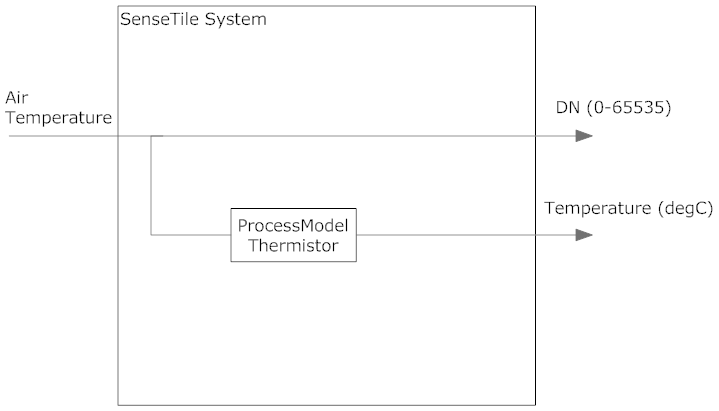
\includegraphics{SensorML_SenseTile_block_design.png}
\caption{Block diagram of SenseTile System process}\label{fig:SensorML_SenseTile_design.png}
\end{figure}


Types
 - SWE -

Count - BigInteger
Quantity - Double

 * Carries an array of int primitives.
 * All data is casted to other types when requested.

public class DataBlockInt extends AbstractDataBlock


mapping packet data to process:packet->sensor process
could be multiple inputs.

\section{BON to SensorML mapping}

\chapter{Design}
High level design
\section{SenseTile Web Service}

DataProducer - use PacketInput stream to access SenseTile observation packets.

DataProvider - provides an RMI interface to the DataProducer to update. Provides a Web Service interface  based on Sensor Observation Service. Not fully as is a very complex interface.

\section{SensorML generation tool}

SensorML BON mapping

BON to Java

Instantiate Java classes with data

Walk Java class and generate sensorml.



\chapter{ Detailed Design and Implementation}

\section{SenseTile WebService}

DataProvider is based on AXIS 2.0/Spring

DataProducer POJO/VastLib/UCD SenseTile Driver Lib

\chapter{Results}




\chapter{ Conclusions and Future Work}

what has been achieved
the weaknesses of your approach

\chapter{References}



\chapter{Appendices}


\newpage
\begin{thebibliography}{99}
\bibitem{SensoMLref}Open Geospatial Consortium Inc., OpenGIS Sensor Model Language (SensorML) Implementation Specification, 2007
\bibitem{BONref}Kim Waldén and Jean-Marc Nerson , "Seamless Object-Oriented Software Architecture", 1995
\end{thebibliography}
\label{endpage}



\end{document}

\end{article}
